\chapter{Planificación y presupuesto}
En este capítulo se va a realizar una planificación del TFG, en la que se
va a explicar la metodología que será utilizada para el desarrollo del proyecto,
se va a estimar el tiempo que se va a tardar en realizar cada tarea del proyecto
y el coste económico que supondría realizar el mismo.

\section{Metodología utilizada}
Para el desarrollo de la aplicación voy a enfocarlo con una \textbf{metodología
tradicional}, ya que es la que más cómoda me resulta y la que más se adapta
a este tipo de proyectos. Además, al ser un proyecto de una sola persona, no es
necesario utilizar una metodología ágil y desde mi punto de vista entorpecería
más el flujo de trabajo.

Las fases de este tipo de metodologías, tal y como se explica en este artículo
sobre metodologías de desarrollo de software \cite{metodologias}, son las siguientes:

\begin{itemize}
  \item \textbf{Análisis}: En esta fase se analiza el problema a resolver y se
  definen los requisitos que debe cumplir la aplicación.
  \item \textbf{Diseño}: En esta fase se diseña la base de datos, la arquitectura
  del sistema y las interfaces de usuario.
  \item \textbf{Implementación}: Esta es la fase en la que se desarrolla la
  aplicación y se implementan las funcionalidades necesarias para satisfacer
  los requisitos.
  \item \textbf{Pruebas}: En la fase de pruebas se comprueba que la aplicación
  cumple con los requisitos y que funciona correctamente.
  \item \textbf{Mantenimiento}: La fase de mantenimiento es en la que se corrigen
  los posibles errores que se encuentren en la aplicación y en la que se pueden
  añadir nuevas funcionalidades a la misma.
\end{itemize}

Tal y como se explica en este otro artículo en el que se comparan las metodologías
\cite{tradicionalesVSagiles}, las ágiles son más adecuadas para proyectos
en los que se trabaja en equipo y se necesita una mayor flexibilidad durante el
desarrollo porque los requisitos pueden cambiar.

En nuestro caso, no es necesario utilizar una metodología ágil porque no hay un equipo de
desarrollo que coordinar en daily meetings, las tareas se realizarán de forma secuencial.
No hay un cliente o stakeholders que puedan cambiar los requisitos de forma
continua, por lo que no es necesario realizar entregas periódicas en sprints como
sí se hace en metodologías ágiles como Scrum. En nuestro caso no habrá feedback del
cliente ni reuniones de retroalimentación, sino que será una única persona la que
se encargará de realizar el control de calidad y verificar que se cumplan los
requisitos de la aplicación.

Para el control de calidad, pruebas y verificación de requisitos, se irá haciendo
de manera continua a medida que se vayan desarrollando las funcionalidades de la
aplicación.

\subsection{Seguimiento del proyecto}
Para el seguimiento del desarrollo de la aplicación se utilizará la herramienta
\textit{Trello} \cite{trello}, perteneciente a la empresa \textit{Atlassian} \cite{atlassian}.
Esta herramienta permite crear tableros de kanban para oraganizar
las tareas pendientes de realizar, las que están en proceso y las que ya se han
realizado. Se puede ver el tablero kanban en la figura \ref{fig:trello}.

En la imágen se puede ver cómo están dividadas las tareas en las tres columnas y
etiquetadas según la etapa a la que pertenecen. Algunas de las tarjetas de tarea
tienen checklist para poder ir marcando las subtareas que se van realizando. Esto
permite tener un seguimiento de las tareas que se van realizando y las que aún
faltan por hacer.

\begin{figure}[H]
  \centering
  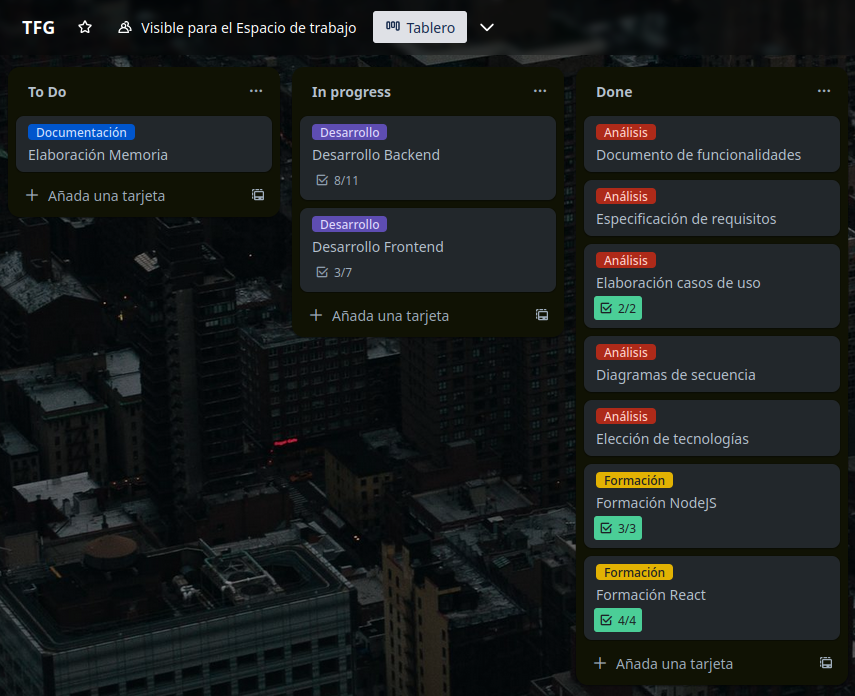
\includegraphics[width=1\textwidth]{trello}
  \caption{Tablero kanban de Trello}
  \label{fig:trello}
\end{figure}


\section{Temporización}
En esta sección se mostrará a través de un diagrama de Gantt la planificación
temporal del proyecto desglosado en tareas. Para ello se ha utilizado la
herramienta \textit{Lucidchart} \cite{lucidchart}.

En la figura \ref{fig:gantt} se muestra el diagrama de Gantt con el desglose de las
tareas que se van a realizar, así como la duración de cada una de ellas en semanas.
Los colores diferencian las etapas del desarrollo del proyecto.

Como se puede ver en el diagrama, el proyecto se va a desarrollar en 16 semanas. La
primera semana se dedicará a la planificación y especificación de los requisitos
que tiene que cumplir la aplicación.

La segunda, tercera y cuarta semana se dedicarán a la elaboración de los casos de uso
y diagramas de secuencia, así como a la elección de las tecnologías que se van a
utilizar para el desarrollo de la aplicación. Esta fase se ha estimado en 3 semanas
ya que es una de las partes más importantes y, al tratarse de una metodología tradicional,
es necesario tener bien definidos todos los requisitos y casos de uso de la aplicación.

Después se ha planficado dejar tres semanas para la formación en las tecnologías que
se van a utilizar para el desarrollo de la aplicación. Esto es orientativo y puede que
durante el desarrollo de la aplicación surjan dudas o problemas que requieran más
tiempo de formación.

Para el desarrollo de la aplicación se ha estimado en unas siete semanas, comenzando
con dos para el desarrollo del backend, otras dos de desarrollo conjunto del backend
y comenzar con el desarrollo del frontend, y las últimas tres semanas para el desarrollo
final del frontend.

La fase de pruebas se irá realizando de forma continua y en paralelo al desarrollo
de la aplicación, además de dedicar una última semana para las pruebas finales de
la misma.

\begin{figure}[H]
  \centering
  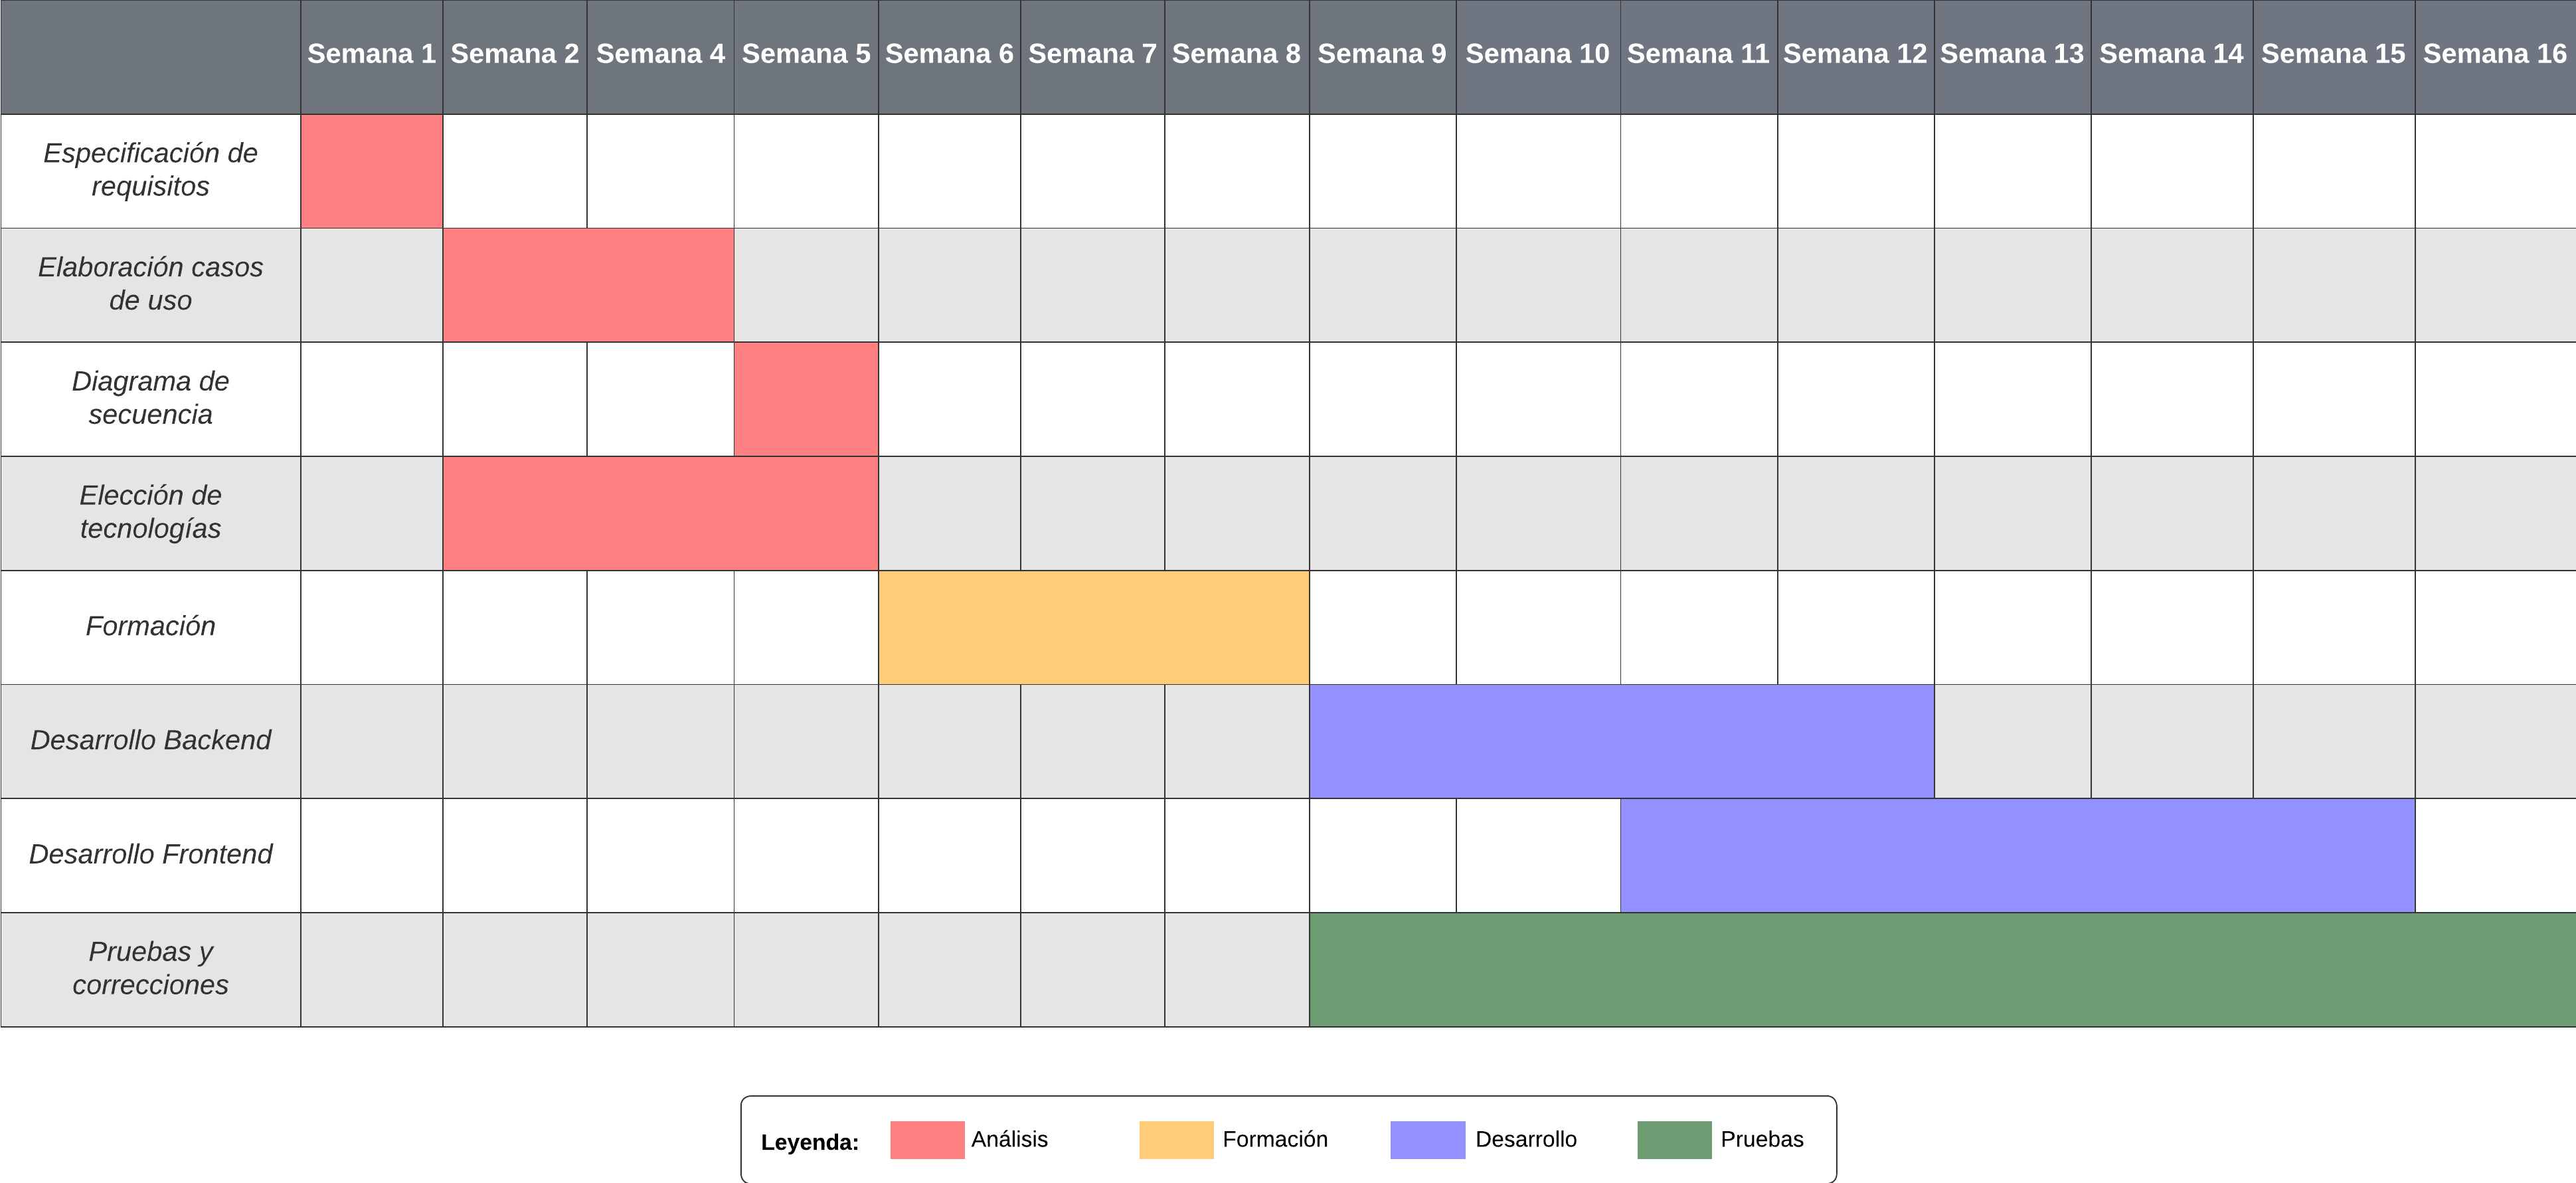
\includegraphics[width=1\textwidth]{gantt}
  \caption{Diagrama de Gantt}
  \label{fig:gantt}
\end{figure}

\section{Presupuesto}
Para elaborar el presupuesto se ha tenido en cuenta el coste de la hora de trabajo
de un ingeniero informático en España, que es de unos 14€/hora \cite{coste-hora}.
Teniendo en cuenta que la duración del proyecto se estima en 16 semanas, y que
se van a dedicar unas 20 horas semanales, el coste del personal sería de \textbf{4480€}.

\vspace{1cm}

En cuanto al coste de los recursos materiales, se ha calculado el coste del portátil
prorrateado en el tiempo que se va a utilizar para el desarrollo del proyecto. El
coste del portátil es de 1799€ \cite{portatil} y teniendo en cuenta que el ciclo de vida de un
portátil es de unos 5 años, el coste prorrateado sería de 29,98€/mes. Por lo tanto,
el coste del portátil durante las 16 semanas de duración del proyecto sería de
\textbf{119,92€}.

\vspace{1cm}

Por último, el coste de los recursos de software utilizados para el desarrollo
del proyecto es de \textbf{0€}, ya que se han utilizado herramientas de software libre.

El editor de texto utilizado es \textit{Visual Studio Code} \cite{vscode} que tiene
licencia \textit{MIT} \cite{mit-license}.

El sistema de control de versiones \textit{Git} \cite{git} tiene licencia
\textit{GPLv2} \cite{gplv2}. Y la plataforma \textit{GitHub} \cite{github} tiene
licencia \textit{MIT} \cite{mit-license}.

Para el desarrollo del backend se va a utilizar \textit{Node.js} \cite{nodejs}
y para el frontend \textit{React} \cite{react}, ambos con licencia
\textit{MIT} \cite{mit-license} también.

\vspace{1cm}

Teniendo en cuenta todo lo anterior, el coste total del proyecto sería de
\textbf{4599,92€}.
